\title{CS 4740 Project 2 Report}
\author{Jaclyn Huang, Dhiraj Gupta, Shannon Joyner [Kaggle Team Name: Jaclyn Huang]}
\date{\today}

\documentclass[12pt]{article}
\usepackage[a4paper, total={7in, 10in}]{geometry}
\usepackage{amsmath}
\usepackage{graphicx}
\usepackage{hyperref}
\hypersetup{
	colorlinks=true,
	urlcolor=blue,
}

\begin{document}
\maketitle


\section{Implementation}
\subsection{Baseline}
For our baseline implementation, we stored the named entity and its label in a set. For every sentence, we checked if each named entity existed in the sentence and if so, gave the named entity that label.
\subsection{HMM}
For HMM, we implemented the Viterbi algorithm as described in lecture (storing backpointers to recover the maximal-probability path). We used the words in sentences as our observations and the BIO labels as our hidden observations. We used a variation of the bigram implementation we made in Project 1. We stored all probabilities in maps. For example, the emission probabilities were a two layer map. To prevent underflow, we stored all probabilities as logs. We implemented plus one smoothing for emission probabilities. To handle unknown words, we also created a backoff map. For every word in the training set, we stored label probabilities for suffixes of up to length 2. This is based on the observation that nouns tend to have similar endings like ``-s", while verbs tend to have endings like ``-ed".
\subsection{MEMM}
We implemented the MEMM similarly to the HMM with respect to algorithms and data structures. The primary difference between the HMM and MEMM comes from the MaxEnt classifier. Unlike an HMM, a MEMM predicts tags by computing the probability $P(c|x)$ with a MaxEnt classifier, where $c$ is a class (in this case a tag) and $x$ is some feature vector. The MaxEnt classifier code we used comes from {\tt nltk}, and all other code is original.

During the training process, we iterate over the data and construct features for each example sentence. Then we pass the features and labels (BIO tags) to the classifier to train. To predict tags for a sentence in the test data, we construct the feature set for a given test sentence and run the Viterbi algorithm on that sentence (the probabilities come from the trained MaxEnt classifier). We used a dictionary to represent features, since the NLTK MaxEnt classifier converts non-boolean feature dictionaries to boolean feature vectors.

Our final feature set is the following vector:
\begin{equation*}
\begin{split}
[&w_{i - 2},\ w_{i - 1},\ w_i,\ w_{i + 1}w_{i + 2},
w_{i - 1}w_i,\ w_iw_{i + 1},\ POS_{i - 2},\ POS_{i - 1},\\
&POS_i,\ w_{i + 1},\ POS_{i + 2}, \ POS_{i - 1}POS_i,\ POS_iPOS_{i + 1},\ NER_{i - 1},\\
&{\tt word\_shape,\ word\_shape\_short,\ has\_number,\ has\_uppercase,}\\
&{\tt has\_hyphen, is\_uppercase}
]
\end{split}
\end{equation*}
where $w_i$ is the $i$th word, $POS_i$ is the part-of-speech tag for $w_i$, and $NER_i$ is the NER tag for $w_i$ (consecutive symbols are bigrams). {\tt word\_shape} refers to the ``format" of a word, so something like ``Donald" would be {\tt Xxxxxx} and something like ``a2z" would be {\tt xdx}.
The intuition behind these features is that they provide a variety of information about the ``neighborhood" of a word whose tag is being predicted. Considering typical sentences and the way a human would approach the sequence tagging task, we believed that both previous and future words as well as corresponding parts of speech would help the MEMM tag correctly. Bigram features were included because named entities often span multiple words, like ``New York Police Department" or ``Donald Trump." Features like ``word shape" and {\tt has\_number} help with unknown words (since we did not use any tools like language model smoothing) and provide strong signals as to the type of entity (e.g. {\tt has\_number} likely indicates a street address or location, not a person). Many of our experiments involve the features used for the MEMM, so see section 3.2 for more detail.
\section{Pre-Processing}
We initially applied the same pre-processing for the MEMM and the HMM. Of course, we also constructed the features described above as part of pre-processing for the MEMM. We omit the detailed explanation, but most of the above features could be computed through a single pass over a given sentence with auxiliary data structures (e.g. constructing bigrams by looking at word pairs and maintaining a dictionary of word to integer mappings). Note that we did not handle unknown words during preprocessing for the MEMM and HMM, since the unknown word features and backoff respectively take care of that. For the MEMM, the features related to words themselves were converted to boolean features, so all of them were set to false.
\section{Experiments}
For all of the following experiments:
\begin{itemize}
	\item We consider a label correct if and only if the entire entity is correct (so if an entity is [New York Yankees] but the system tags [New York] then it's considered incorrect).
	\item The validation set was constructed from a random sampling of 20\% of the training data, and the training set was the remaining 80\%. We only sampled once, so the validation and training sets remained fixed for all experiments.
\end{itemize}
As a comparison point, the following table shows results from our baseline model in Section 1.1 on the validation set:
\begin{center}
	\begin{tabular}{|c|c|c|c|c|}
		\hline
		\textbf{Metric/Category} & {\tt LOC} & {\tt MISC} & {\tt ORG} & {\tt PER}\\
		\hline
		Precision & 0.65 & 0.59 & 0.34 & 0.26\\
		\hline
		Recall & 0.54 & 0.57 & 0.28 & 0.23\\
		\hline
		F1 Score & 0.59 & 0.58 & 0.31 & 0.25\\
		\hline
	\end{tabular}
\end{center}
\subsection{HMM}
The first experiment we ran was implementing the backoff probabilites. Originally we just implemented plus 1 smoothing and chose a small epsilon number for unknown words. The results for this method are below:
\begin{center}
	\begin{tabular}{|c|c|c|c|c|}
		\hline
		\textbf{Metric/Category} & {\tt LOC} & {\tt MISC} & {\tt ORG} & {\tt PER}\\
		\hline
		Precision & 0.83 & 0.76 & 0.73 & 0.84 \\
		\hline
		Recall & 0.73 & 0.43 & 0.44 & 0.54 \\
		\hline
		F1 Score & 0.78 & 0.55 & 0.55 & 0.66\\
		\hline
	\end{tabular}
\end{center}
However, we wanted a better model for unknown words since all unknown words are unlikely to have the same probabilities. So we implemented suffix probabilities with the theory that this would give a better estimation for unknown words. Specifically, when encountering an unknown word we considered its suffix, since (for example) nouns tend to end in ``-s" and verbs tend to end in ``-ed", so it's unlikely that a word ending in ``-ed" is part of an entity, which is usually a noun. The results after implementing a suffix probability-based backoff are as follows:
\begin{center}
	\begin{tabular}{|c|c|c|c|c|}
		\hline
		\textbf{Metric/Category} & {\tt LOC} & {\tt MISC} & {\tt ORG} & {\tt PER}\\
		\hline
		Precision & 0.84 & 0.80 & 0.74 & 0.84\\
		\hline
		Recall & 0.78 & 0.47 & 0.48 & 0.58\\
		\hline
		F1 Score & 0.81 & 0.59 & 0.58 & 0.68\\
		\hline
	\end{tabular}
\end{center}
These results are better in almost every aspect, which is expected. Since unknown words are equally likely to be any of the 4 categories of entity, it makes sense that we see a performance improvement across the range of categories rather than in one specific place. We initially anticipated a greater improvement in performance with this method, but it might be the case that our validation set did not contain many unknown words and so the impact of the backoff was minimized.   
\subsection{MEMM}
The experiments we ran using the MEMM all involved differing feature sets, since the feature set is the key detail which affects performance of a MEMM. Our initial feature template does not contain information about structure of the words: 
\begin{equation*}
\begin{split}
[&w_{i - 2},\ w_{i - 1},\ w_i,\ w_{i + 1}w_{i + 2},
w_{i - 1}w_i,\ w_iw_{i + 1},\ POS_{i - 2},\ POS_{i - 1},\\
&POS_i,\ w_{i + 1},\ POS_{i + 2}, \ POS_{i - 1}POS_i,\ POS_iPOS_{i + 1},\ NER_{i - 1}
]
\end{split}
\end{equation*}
As a result, unknown words are not represented properly since they tend to be all zeros on the boolean features. We expected that this initial feature set would have performance comparable to our HMM, since it accounts for more information but does not handle the problem of unknown words. Examining the precision and recall for this implementation, we find the following:
\begin{center}
	\begin{tabular}{|c|c|c|c|c|}
		\hline
		\textbf{Metric/Category} & {\tt LOC} & {\tt MISC} & {\tt ORG} & {\tt PER}\\
		\hline
		Precision & 0.87 & 0.83 & 0.76 & 0.81\\
		\hline
		Recall & 0.74 & 0.32 & 0.59 & 0.66\\
		\hline
		F1 Score & 0.80 & 0.47 & 0.67 & 0.73\\
		\hline
	\end{tabular}
\end{center}
We also decided to submit this system to Kaggle, where it scored 0.78566. 

To improve these results, we experimented with the template for handling unknown words as suggested in the textbook. The results for this feature template:
\begin{equation*}
\begin{split}
[&w_{i - 2},\ w_{i - 1},\ w_i,\ w_{i + 1}w_{i + 2},
w_{i - 1}w_i,\ w_iw_{i + 1},\ POS_{i - 2},\ POS_{i - 1},\\
&POS_i,\ w_{i + 1},\ POS_{i + 2}, \ POS_{i - 1}POS_i,\ POS_iPOS_{i + 1},\ NER_{i - 1},\\
&{\tt word\_shape,\ word\_shape\_short,\ has\_number,\ has\_uppercase,}\\
&{\tt has\_hyphen, is\_uppercase}
]
\end{split}
\end{equation*}
are here:
\begin{center}
	\begin{tabular}{|c|c|c|c|c|}
		\hline
		\textbf{Metric/Category} & {\tt LOC} & {\tt MISC} & {\tt ORG} & {\tt PER}\\
		\hline
		Precision & 0.88 & 0.84 & 0.80 & 0.83\\
		\hline
		Recall & 0.65 & 0.21 & 0.49 & 0.55\\
		\hline
		F1 Score & 0.75 & 0.33 & 0.60 & 0.66\\
		\hline
	\end{tabular}
\end{center}
Surprisingly, the results here are slightly worse than the results from the previous step. However, this model performed better according to Kaggle. The previous model scored about 0.78, while this new model scored about 0.82. 

We noted that the new features tend to become very informative when predicting whether a word should \emph{not} be associated with a certain label. For instance, if a word does not contain an uppercase letter, then it is very unlikely to be tagged with either {\tt B-LOC}, {\tt B-MISC}, {\tt B-ORG}, or {\tt B-PER}. Indeed, all of them are ranked among the 30 most informative features (according to the coefficients learned by the logistic regression).

We suspect the discrepancy between Kaggle scores and our own experiments is because of the way we selected the validation set. Since this model has better handling for unknown words, if we stratified the validation set (as opposed to sampling randomly), we might have observed better performance from this model. For example, some of the training data is about baseball while other parts of it seem like current events. If we trained on baseball and validated on current events, this model would likely perform better than the previous model (since it would be able to identify unseen people, locations, and so on more accurately than the previous model). 

Given that these features were ranked as so informative, we also tried a feature set consisting mainly of these features: 
\begin{equation*}
\begin{split}
[
&NER_{i - 1}, {\tt word\_shape,\ word\_shape\_short,\ has\_number,\ has\_uppercase,}\\
&{\tt has\_hyphen, is\_uppercase}
]
\end{split}
\end{equation*}
The results were very poor:
\begin{center}
	\begin{tabular}{|c|c|c|c|c|}
		\hline
		\textbf{Metric/Category} & {\tt LOC} & {\tt MISC} & {\tt ORG} & {\tt PER}\\
		\hline
		Precision & 0.61 & 1.0 & 1.0 & 0.00\\
		\hline
		Recall & 0.04 & 0.003 & 0.003 & 0.00\\
		\hline
		F1 Score & 0.08 & 0.01 & 0.01 & 0.00\\
		\hline
	\end{tabular}
\end{center}
The problem is likely that these features don't provide enough information to correctly classify. The context of previous words, parts of speech and the words themselves provide important clues as to whether or not a sequence of words represents an entity. So these features may be important, but in the absence of other features lack the necessary information to correctly tag word sequences. It might also be that many of the entities were previously seen, so using only features whose primary purpose is to describe unknown words doesn't provide much value in tagging familiar sentences. 

\section{Results}
Our final system was the MEMM with feature set described in 1.1. Our evaluation process was as described in 1.3 (Experiments). Additionally, the test dataset performance was measured by the mean F1-score among the 4 tag types on half of the test set provided to us. The Kaggle score was 0.82401, which is noticeably better than the results achieved in our own experiments (see second table in 1.3.2 for final results). We attribute this to the increased number of iterations we ran the MaxEnt classifier for to make the final submission. 

For comparison purposes, here are the mean precision, recall, and F1 score of our baseline system, HMM, and final MEMM across all 4 types of entity:
\begin{center}
	\begin{tabular}{|c|c|c|c|c|}
		\hline
		\textbf{Model/Metric} & Precision & Recall & F1 Score & Kaggle Score\\
		\hline
		Baseline & 0.46 & 0.41 & 0.43 & 0.37\\
		\hline
		HMM & 0.81 & 0.58 & 0.67 & 0.70\\
		\hline
		MEMM & 0.84 & 0.46 & 0.59 & 0.82\\
		\hline
	\end{tabular}
\end{center}
Our HMM and MEMM both vastly outperform the baseline (see section 1 for details on each system). Notice that the HMM outperforms the MEMM by some of these metrics; see section 5 for a detailed discussion of why this might have happened. Given that our baseline basically memorizes seen entities and predicts them, it's no surprise that it's far worse at tagging than our other systems. 

To get a sense of the kinds of errors our final tagger made, we examined the precision and recall on the development set, which was broken down by category (refer to the second table under Section 3.2, at the bottom of page 3). We see that {\tt MISC} was by far the worst category in part because the recall is so poor. This intuitively makes sense, since the {\tt MISC} category likely has a lot of diverse examples, and ones that haven't yet been seen by the tagger. So the probability of any given word or set of words belonging to {\tt MISC} would be quite low. In fact, examining the results as a whole we see that recall is significantly worse than precision across the board. The low recall indicates that the classifier is ``too strict" in predicting entities, and when coupled with the high precision seems to imply that the classifier makes good predictions for a subset of words or phrases that are actually entities. So one possible fix for this problem is finding a feature set which makes the classifier more liberal in predicting entity tags, rather than {\tt O}. For example, it might be better to cut out some features like POS bigrams in order to create a less strict classifier. We also see that {\tt ORG} is the worst class in terms of precision. We suspect this is because {\tt ORG} is a particularly ``confusing" category. For example, baseball teams are organizations, but a prefix of their full name (e.g. [New York] Yankees) is generally a location. As a result, {\tt ORG} word sequences are the most likely to be output \emph{incorrectly}, not just skipped over. One possible fix for this problem would be to add trigram features, but this runs the risk of overcomplicating the model and yielding overall worse results. 

\section{HMMs vs. MEMMs}
For better comparison purposes, here are the results for our final HMM (left) and MEMM (right). The Kaggle scores were 0.70460 and 0.82401 respectively.
\begin{center}
	\begin{tabular}{|c|c|c|c|c|}
		\hline
		\textbf{Metric/Category} & {\tt LOC} & {\tt MISC} & {\tt ORG} & {\tt PER}\\
		\hline
		Precision & 0.84 & 0.80 & 0.74 & 0.84\\
		\hline
		Recall & 0.78 & 0.47 & 0.48 & 0.58\\
		\hline
		F1 Score & 0.81 & 0.59 & 0.58 & 0.68\\
		\hline
	\end{tabular}
	\begin{tabular}{|c|c|c|c|c|}
		\hline
		\textbf{Metric/Category} & {\tt LOC} & {\tt MISC} & {\tt ORG} & {\tt PER}\\
		\hline
		Precision & 0.88 & 0.84 & 0.80 & 0.83\\
		\hline
		Recall & 0.65 & 0.21 & 0.49 & 0.55\\
		\hline
		F1 Score & 0.75 & 0.33 & 0.60 & 0.66\\
		\hline
	\end{tabular}
\end{center}
As expected, the MEMM performed better on the sequence-tagging task than the HMM with respect to Kaggle score. Surprisingly, the performance estimation using our validation set indicates the HMM outperforms the MEMM. This discrepancy could be caused by several factors: first, the Kaggle submission for the MEMM used many more training iterations than the experimentation (for computational reasons). As a result, the MEMM should perform better on Kaggle than in experiments. As previously discussed, our method of creating the validation set might have also contributed to this pattern. Since we did not explicitly stress prediction on unknown words (via stratifying the training data deliberately) these models were not evaluated as aggressively on unknown words. From our MEMM experiments, we see that the features relating to unknown words are highly significant to the MaxEnt classifier. So perhaps if we constructed the validation set differently, we would observe that the MEMM outperforms the HMM according to these metrics. 

The HMM and MEMM have similar trends with respect to errors. Both have the lowest precision on {\tt ORG}. We suspect this is because {\tt ORG} is a particularly ``confusing" category. For example, baseball teams are organizations, but a prefix of their full name (e.g. [New York] Yankees) is generally a location. As a result, {\tt ORG} word sequences are the most likely to be output \emph{incorrectly}, not just skipped over. However, {\tt MISC} is the worst category with respect to recall. This is probably because {\tt MISC} is the most diverse category and might contain unseen examples, which are likely to be tagged as {\tt O} since they are harder to identify as entities. 

It makes sense that the HMM and MEMM exhibit similar error patterns. The main difference between the HMM and MEMM is that the MEMM can draw on a greater amount of information to make its tagging decisions, but none of the feature vectors we constructed would improve an MEMM over an HMM only in a specific category. Features like part of speech or preceding words should help in all entity categories since any of them could span multiple words, and most of them would likely be nouns. We also believe that the MEMM's unknown word handling is much better than the HMM's unknown word handling, but unknown words should be uniformly distributed across all 4 categories of entity. As a result, we would expect to observe a better performance over all 4 categories by the MEMM. We've already discussed why this isn't the case for our own metrics, but the Kaggle scores support this conclusion.
  
\section{Competition Score}
Our Kaggle team name was ``Jaclyn Huang" and our competition score was 0.82401. Below is the image of the Kaggle submission:
\begin{center}
	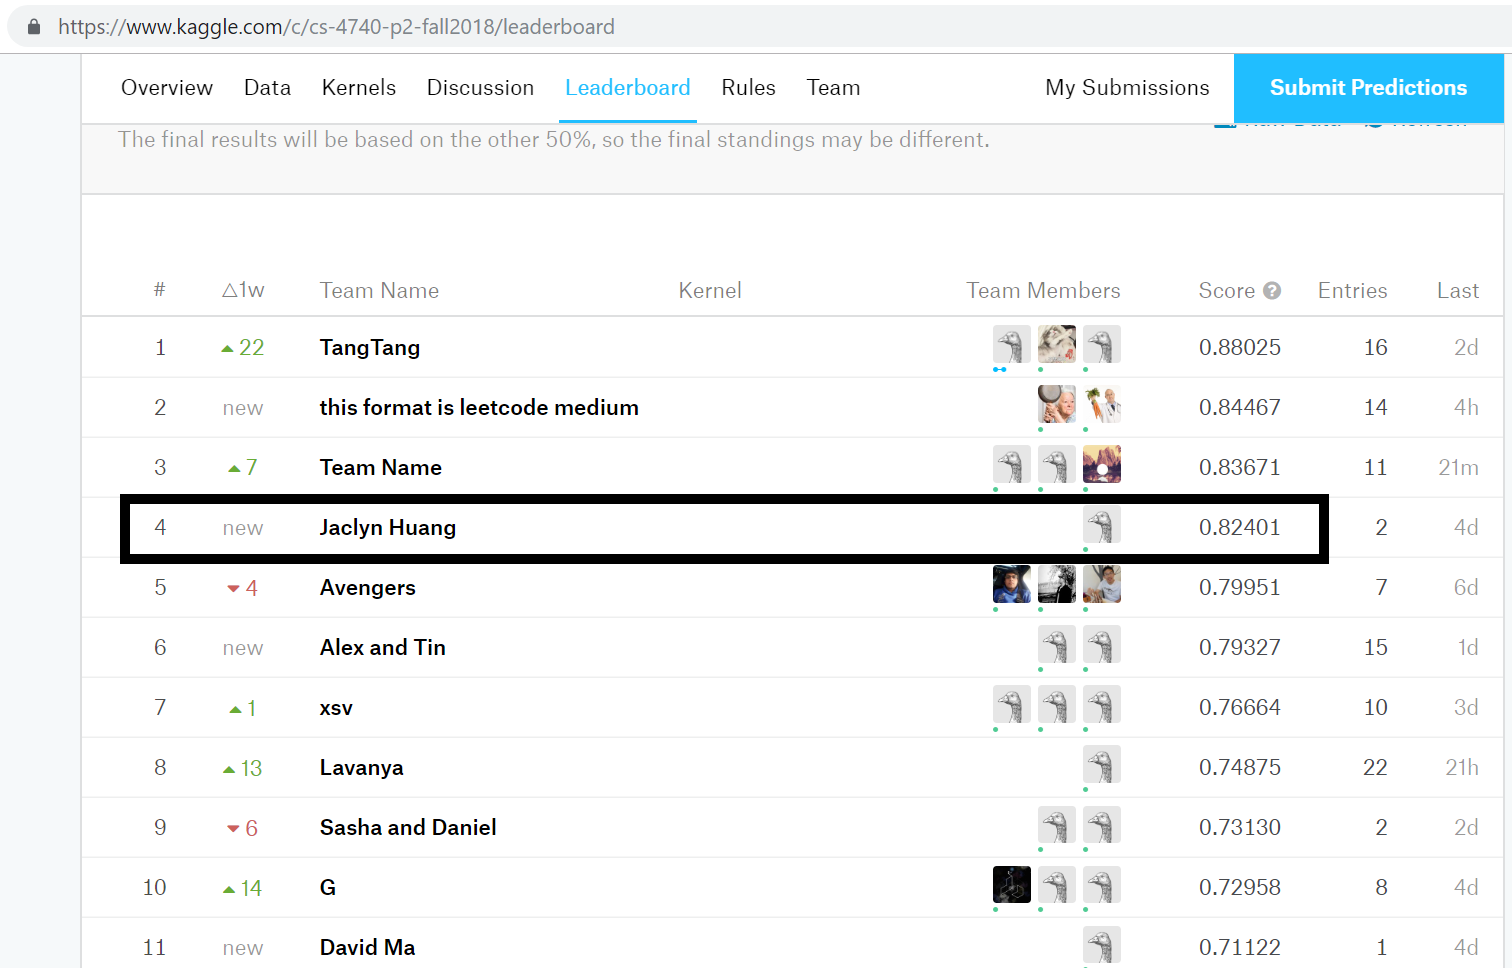
\includegraphics[scale=0.25]{kaggle.png}
\end{center}
We mistakenly made other submissions under different team names but the team in this report is the correct, final one. 

\section{Individual Member Contribution}
\begin{itemize}
	\item Shannon: HMM and baseline implementation
	\item Jaclyn: MEMM implementation
	\item Dhiraj: Experiments, error analysis, HMM and MEMM comparison
\end{itemize}
\end{document}
